\documentclass[border=10pt]{standalone}
\usepackage{pgfplots}
\pgfplotsset{compat=1.17}
\begin{document}
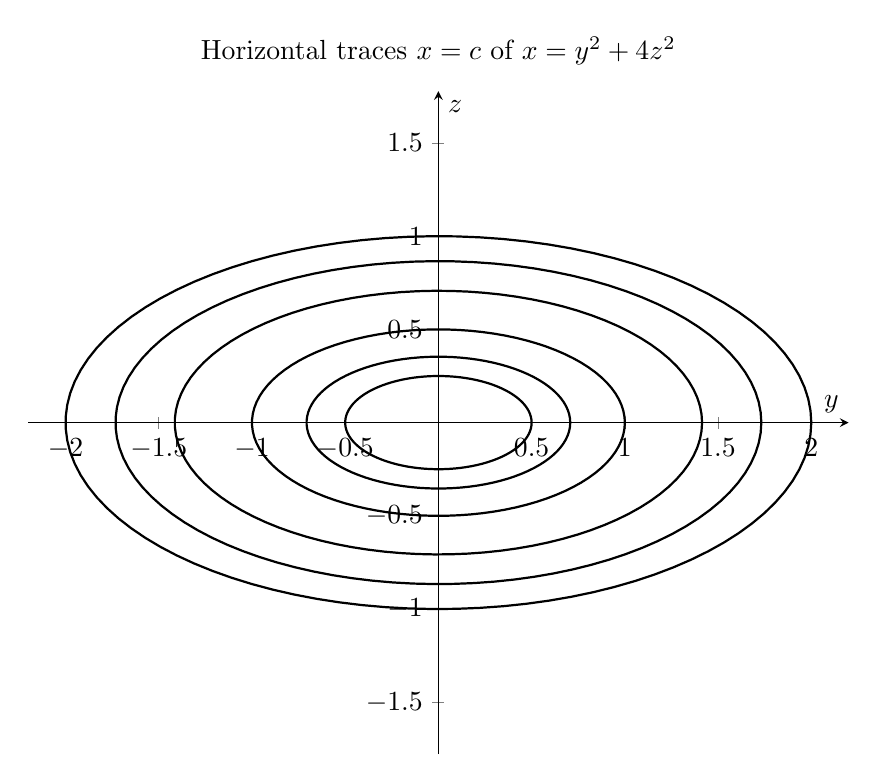
\begin{tikzpicture}
\begin{axis}[
    xlabel={$y$}, ylabel={$z$},
    xmin=-2.2, xmax=2.2,
    ymin=-1.2, ymax=1.2,
    axis equal,
    axis lines=middle,
    width=12cm,
    height=10cm,
    title={Horizontal traces $x=c$ of $x=y^2+4z^2$}
]
\pgfplotsinvokeforeach{0.25,0.5,1,2,3,4}{
    \addplot[thick, domain=0:360, samples=100, variable=\t]
        ({sqrt(#1)*cos(\t)}, {sqrt(#1)/2*sin(\t)});
}
\end{axis}
\end{tikzpicture}
\end{document}
